\section{Silicon --- Disentangled MLWFs}
\label{sec3:silicon}
\begin{itemize}
\item Outline: {\it Obtain disentangled MLWFs for the valence and low-lying conduction states of Si. Plot the interpolated bandstructure.}
\end{itemize}

\begin{figure}[h!]
\centering
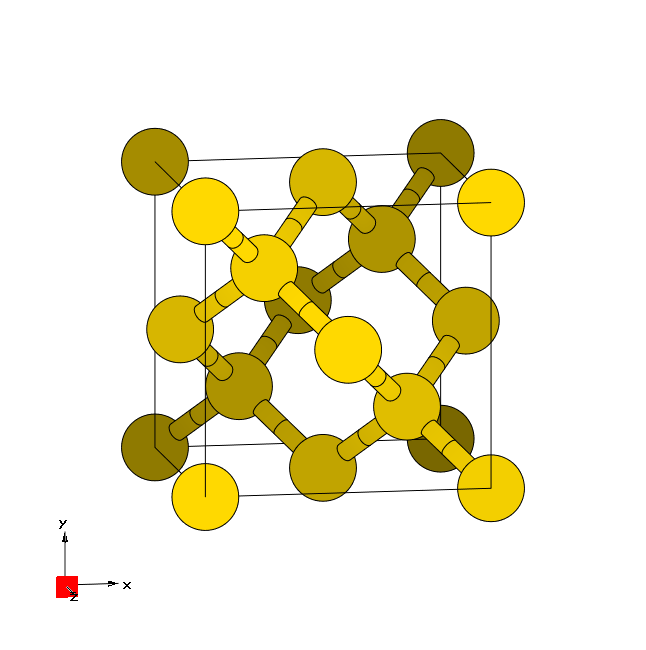
\includegraphics[width=0.25\columnwidth,trim={45pt 45pt 55pt 55pt},clip]{figure/example03/silicon.png}
\caption{Unit cell of Silicon crystal plotted with the \xcrysden{} program.}
\label{fig3.0}
\end{figure}


\begin{enumerate}
	\item {\it Inspect the output file \tt{silicon.wout}.} 

	Starting from 4 $sp3$ orbitals on each Silicon atom we obtain two sets of 4 WFs, all with the same spread, that show the $sp3$ character one would expect from symmetry considerations. A summary of the wannierisation is given in tab.\ref{tab3.1}. At the end of the {\tt .wout} file you should find the info on the final state of the minimization, here we show an extract of the output file
	\begin{tcolorbox}[sharp corners,boxrule=0.5pt]
	{\small
	\begin{verbatim}
	 Final State
  WF centre and spread    1  ( -0.460754, -0.460711, -0.460767 )     1.81241746
  WF centre and spread    2  ( -0.460743,  0.460722,  0.460718 )     1.81246400
  WF centre and spread    3  (  0.460703, -0.460761,  0.460685 )     1.81248774
  WF centre and spread    4  (  0.460704,  0.460724, -0.460764 )     1.81244947
  WF centre and spread    5  (  1.810128,  1.810112,  1.810113 )     1.81247628
  WF centre and spread    6  (  1.810097,  0.888662,  0.888617 )     1.81242110
  WF centre and spread    7  (  0.888640,  1.810140,  0.888660 )     1.81240614
  WF centre and spread    8  (  0.888643,  0.888652,  1.810090 )     1.81245230
  Sum of centres and spreads (  5.397417,  5.397539,  5.397353 )    14.49957450
 
         Spreads (Ang^2)       Omega I      =    11.849193709
        ================       Omega D      =     0.105470243
                               Omega OD     =     2.544910550
    Final Spread (Ang^2)       Omega Total  =    14.499574503
 ------------------------------------------------------------------------------
	\end{verbatim}
	}
	\end{tcolorbox}
	\begin{table}[b!]
	\centering
        \caption{Converged values of the components of spread functional and their sum, given in \angsqd{}.}
	\label{tab3.1}
	\begin{tabular}{@{} lllll @{}}\toprule[1.5pt]
	MP mesh & $\Omega$ & $\Omega\tinysub{I}$ & $\Omega\tinysub{OD}$ & $\Omega\tinysub{D}$ \\\midrule
	$4\times4\times4$ & 14.5 & 11.849 & 2.545 & 0.105 \\\bottomrule[1pt]
	\end{tabular}
	\end{table}
	\item {\it Plot the energy bands.}

	As can be seen from DFT bandstructure plot in the \Wannier{} tutorial, that we report here, \cf{} \Fig{fig3.1}, the four lower valence bands are separated in energy from the higher conduction states (there is however an indirect band gap). The Fermi level lies inside the gap, making crystalline Silicon a semiconductor.

	The path in $\bfk$-space given in the tutorial (L-$\Gamma$-X-K-$\Gamma$) and shown in \Fig{fig3.2}-(a)-top is the following
	{\tt
	\begin{quote}
begin kpoint\_path

L 0.50000  \phantom{-}0.50000 0.5000 G \phantom{-}0.00000  0.00000 0.0000

G 0.00000  \phantom{-}0.00000 0.0000 X \phantom{-}0.50000  0.00000 0.5000

X 0.50000 -0.50000 0.0000 K 0.37500 -0.37500 0.0000

K 0.37500 -0.37500 0.0000 G 0.00000  \phantom{-}0.00000 0.0000

end kpoint\_path
	\end{quote}}
	which gives the bandstructure shown in \Fig{fig3.2}-(a)-bottom. 

	\item[Extra :] {\it Try plotting along different paths.} 

	Another path usually used for Silicon is \mbox{W-$\Gamma$-X-W-L-$\Gamma$} shown in \Fig{fig3.1}-(b)-top and the corresponding bands are shown in \Fig{fig3.2}-(b)-bottom. To obtain this path you need to replace the previous {\tt kpoint\_path} block with the following block
	{\tt 
	\begin{quote}
	begin kpoint\_path

	W  \phantom{-}0.25000  0.75000  \phantom{-}0.50000 G  \phantom{-}0.00000   0.00000  \phantom{-}0.00000

	G  \phantom{-}0.00000  0.00000  \phantom{-}0.00000 X  \phantom{-}0.50000  0.50000  \phantom{-}0.00000

	X  \phantom{-}0.50000  0.50000  \phantom{-}0.00000 W -0.25000  0.25000 -0.25000

	W -0.25000  0.25000 -0.25000 L  \phantom{-}0.00000  0.50000  \phantom{-}0.00000

	L  \phantom{-}0.00000  0.50000  \phantom{-}0.00000 G  \phantom{-}0.00000  0.00000  \phantom{-}0.00000

    end kpoint\_path
	\end{quote}} 

	\begin{figure}[t!]
	\centering
	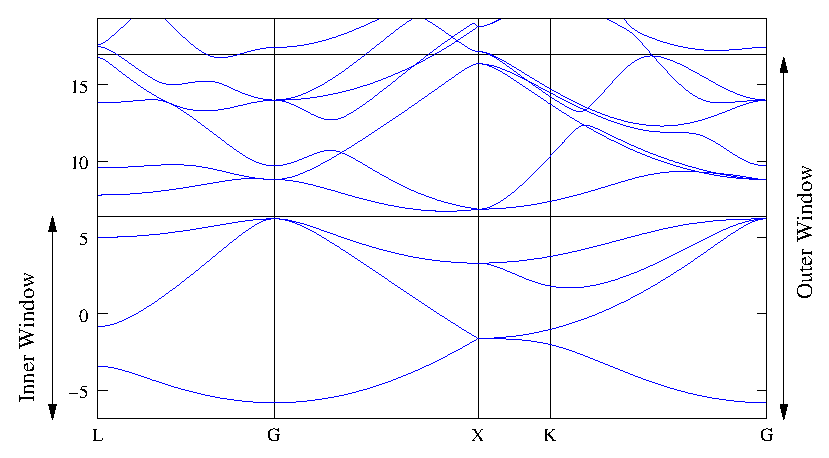
\includegraphics[width=0.7\columnwidth]{figure/example03/si.eps}
	\caption{Bandstructure of Silicon showing the position of the Fermi level and of the inner and outer windows. Both the 4 valence bands and the 4 low-lying conduction bands are included in the calculation.}\label{fig3.1}
	\end{figure}

	\begin{figure}[h!]
	\centering
	\subfloat[]{\stackinset{c}{-.09\textwidth}{b}{+.06\textwidth}
	{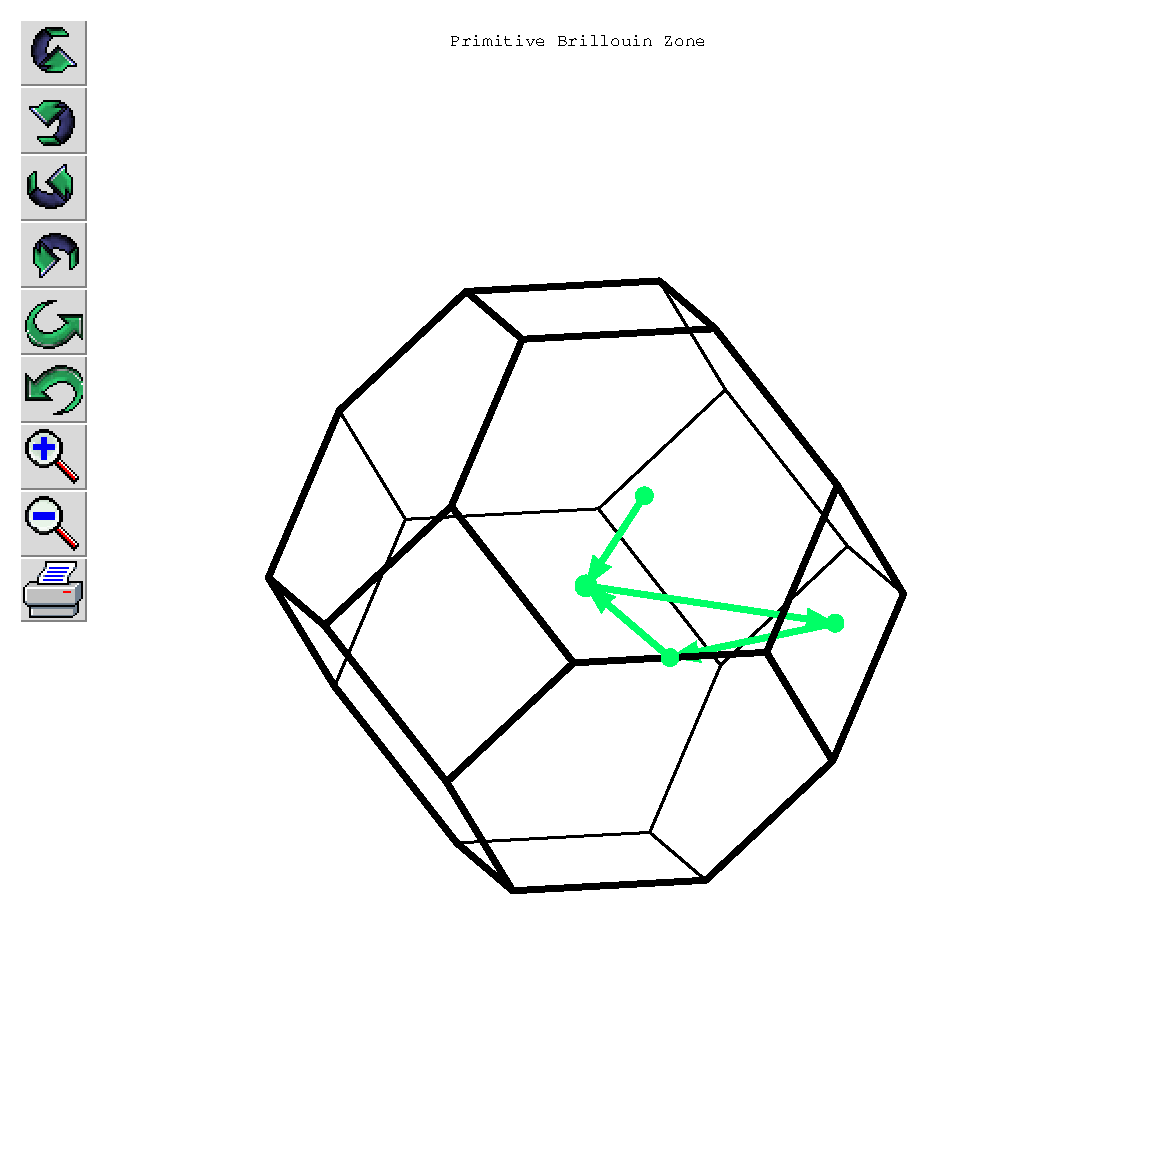
\includegraphics[width=0.09\textwidth,trim={1.5cm 0cm 2cm 3cm},clip]{figure/example03/silicon_bs1_nopts.eps}}
	{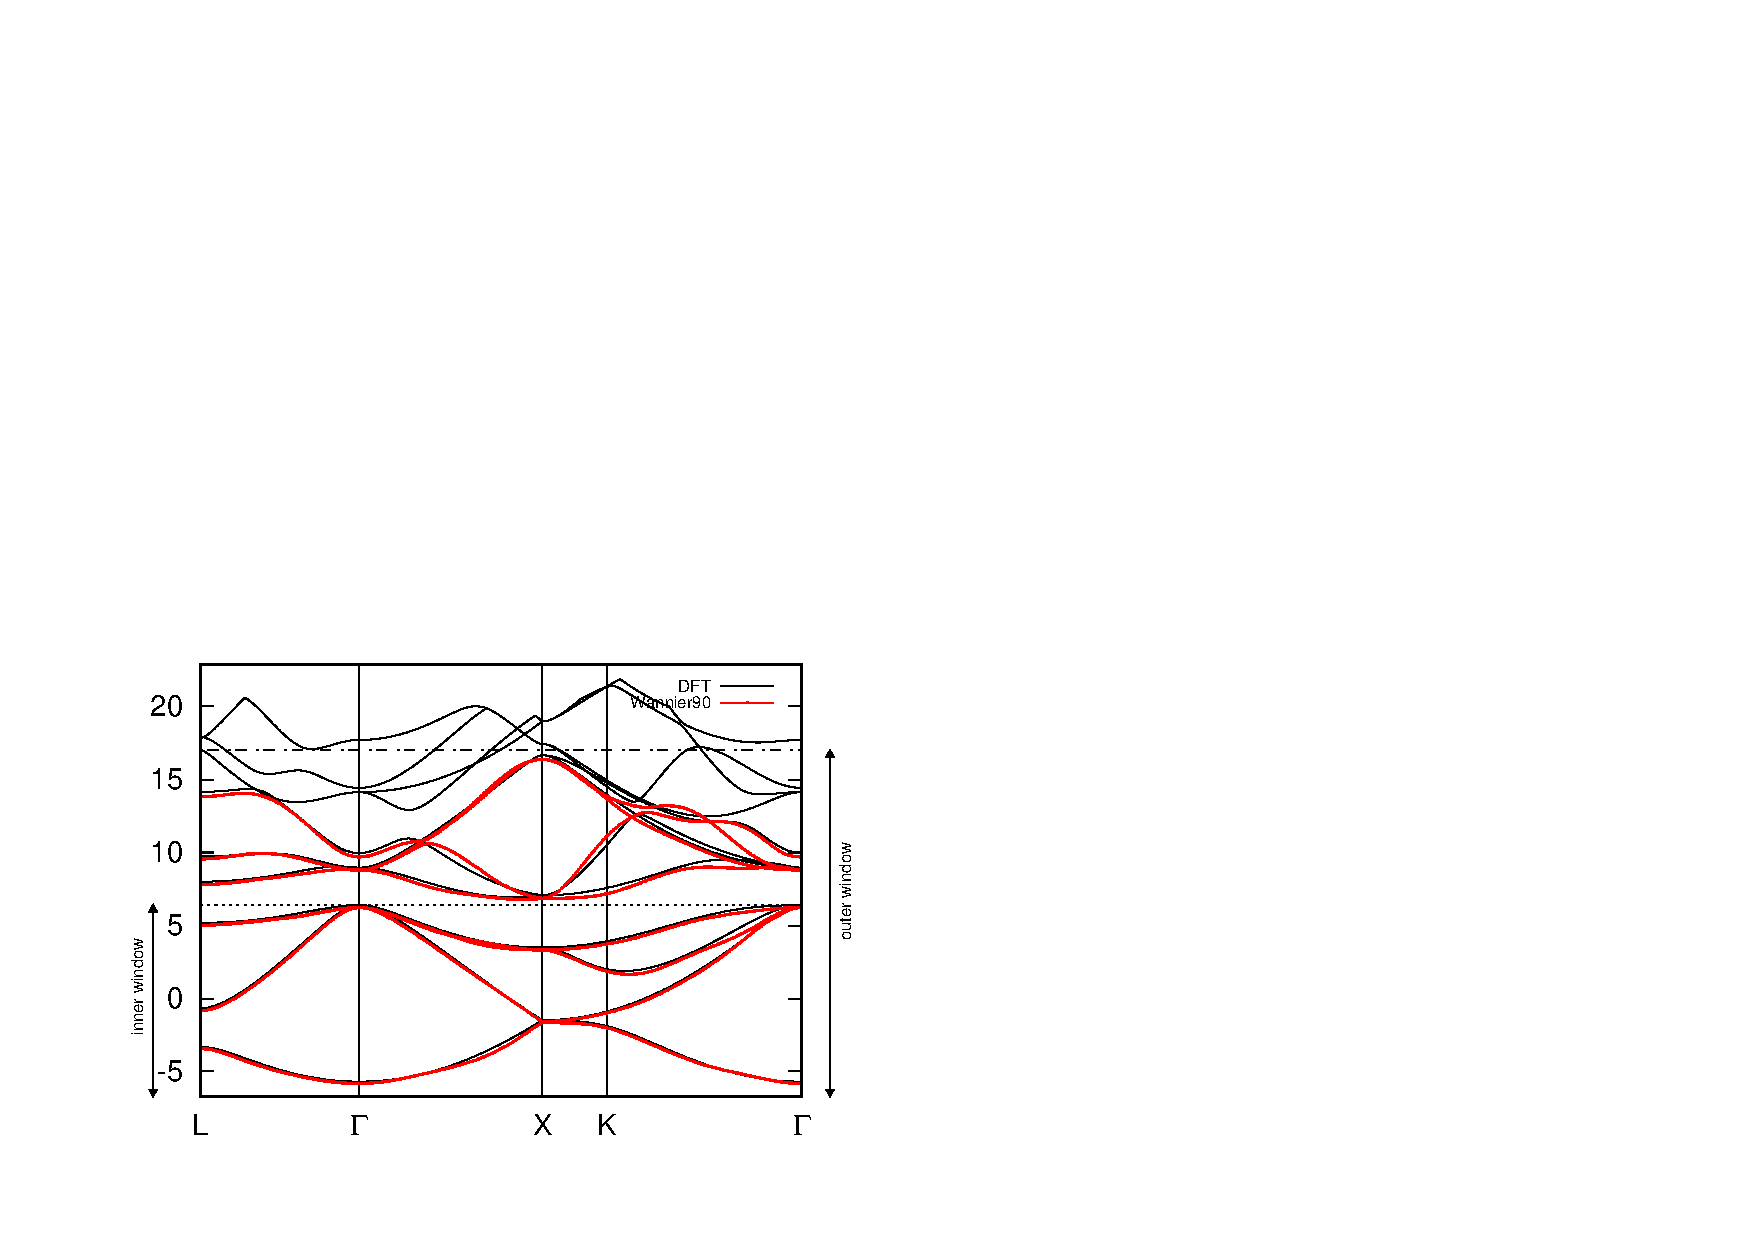
\includegraphics[width=0.6\columnwidth,trim={2.cm 1cm 15cm 11cm},clip]{figure/example03/silicon_DFT_W90_bs_path1.pdf}}}\\
	\centering
	\subfloat[]{\stackinset{c}{-.09\textwidth}{b}{+.06\textwidth}
	{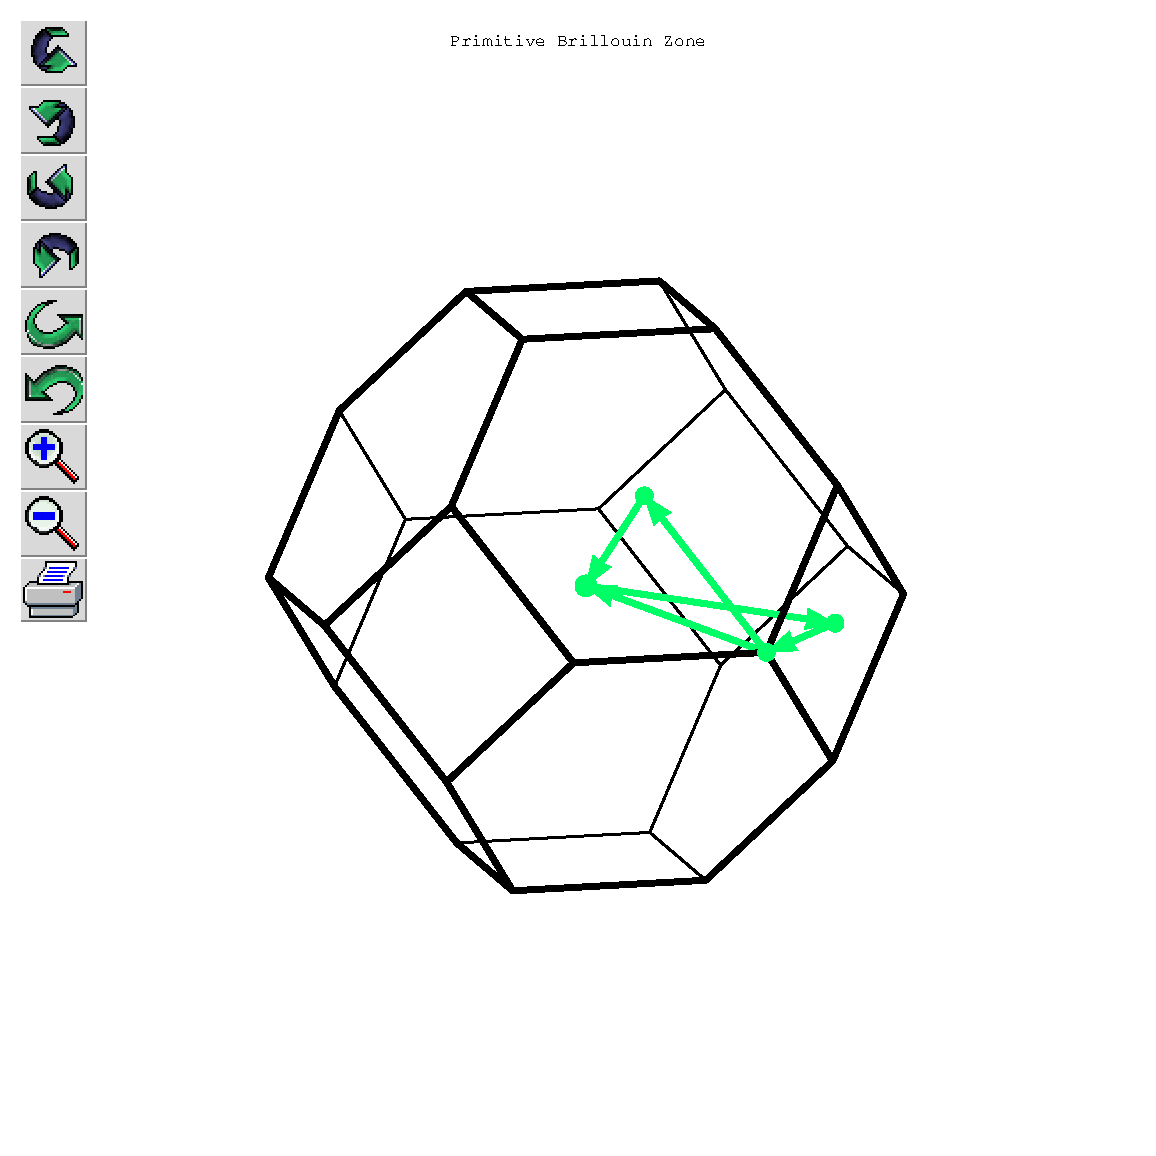
\includegraphics[width=0.09\textwidth,trim={1.5cm 0cm 2cm 3cm},clip]{figure/example03/silicon_bs2_nopts.eps}}
	{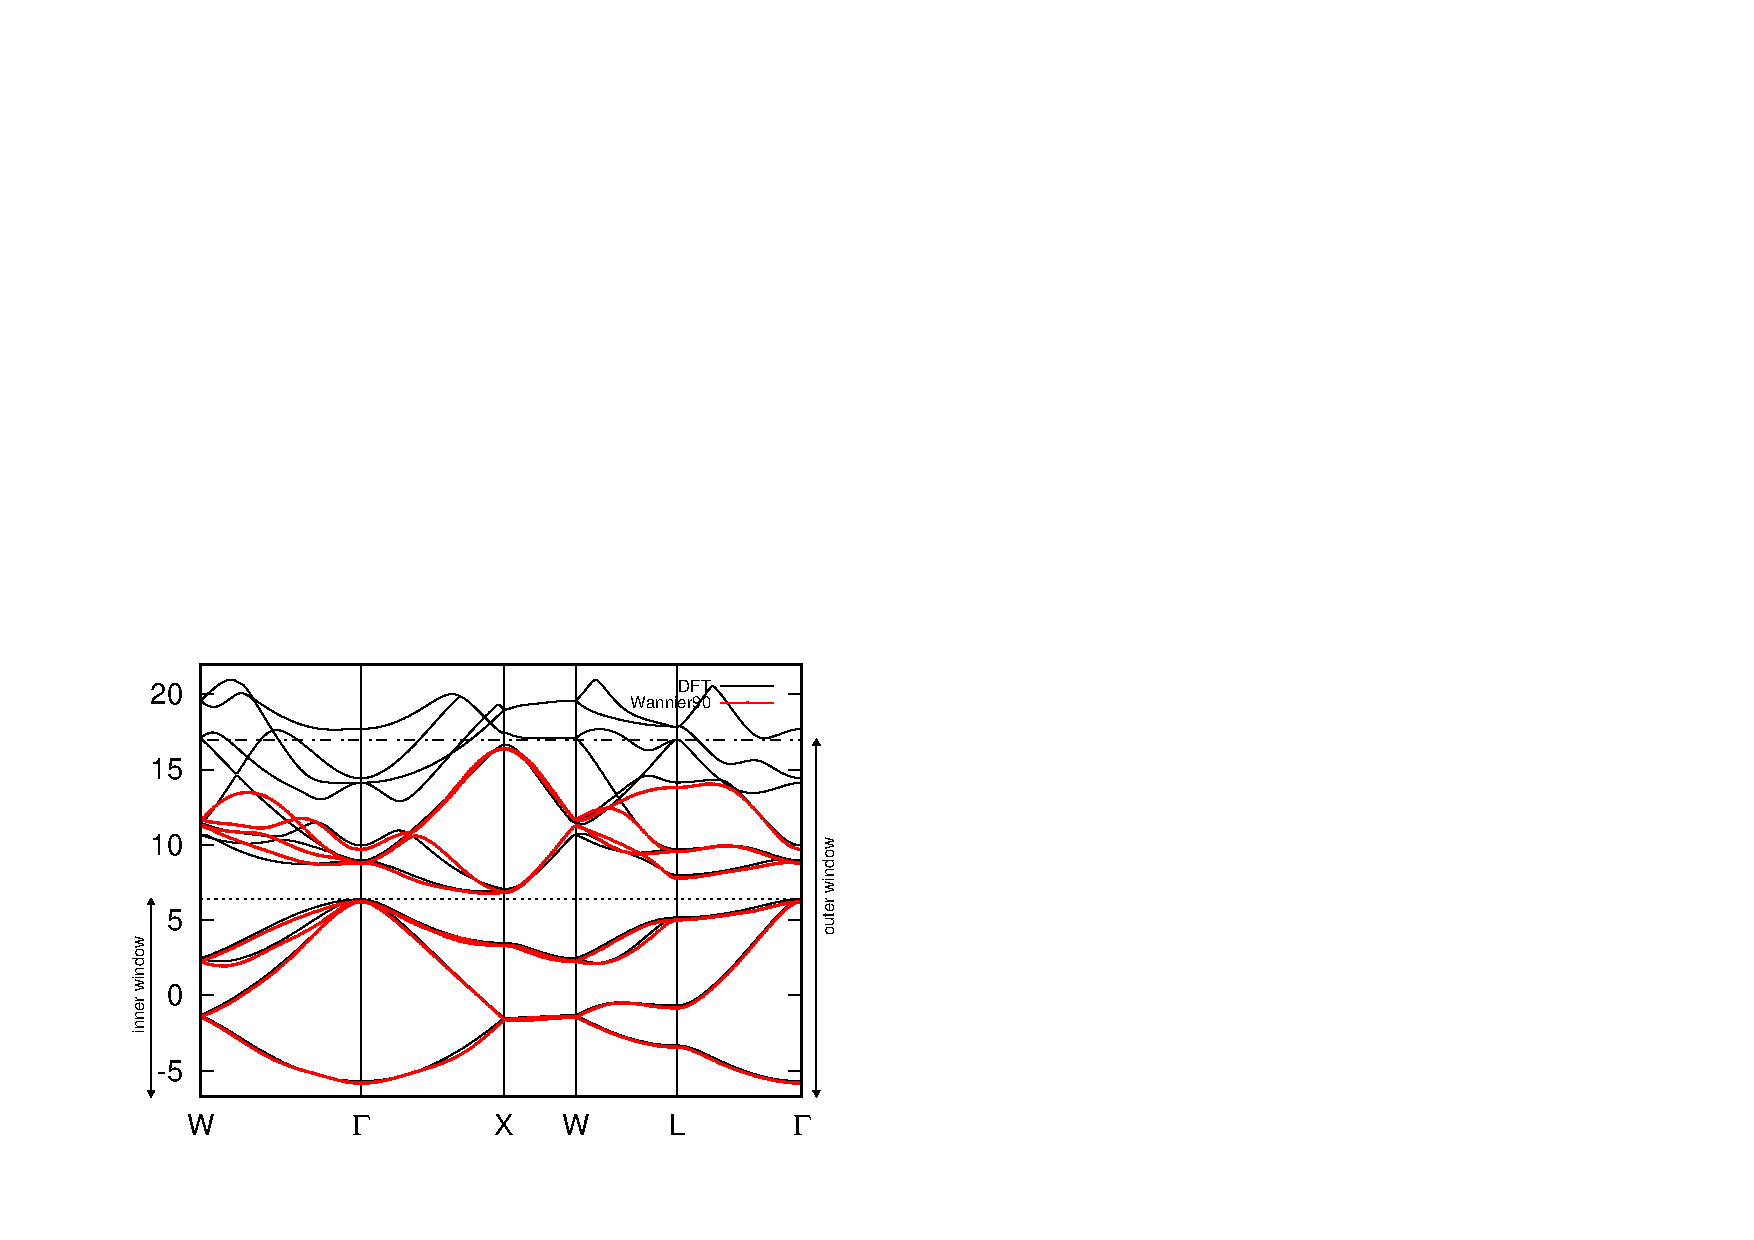
\includegraphics[width=0.6\columnwidth,trim={2.cm 1cm 15cm 11cm},clip]{figure/example03/silicon_DFT_W90_bs_path2.pdf}}}
	\caption{Bandstructure of Silicon showing the position of the Fermi level and of both the inner and outer windows. The 4 valence bands together with the 4 low-lying conduction bands are included in the calculation. Panel a) Interpolation with Wannier90 on the \mbox{L-$\Gamma$-X-K-$\Gamma$} path in $\bfk$ space (red dots) and DFT reference bandstructure (solid black). Panel b) Interpolation with Wannier90 on the \mbox{W-$\Gamma$-X-W-L-$\Gamma$} path in $\bfk$ space (red dots) and DFT reference bandstructure (solid black).}\label{fig3.2}
	\end{figure}

\end{enumerate}
